\documentclass[crop,border=2pt]{standalone}

\usepackage{mathtools}
\usepackage{tikz}
\usetikzlibrary{positioning,scopes,arrows,shapes,decorations.pathreplacing}

\begin{document}
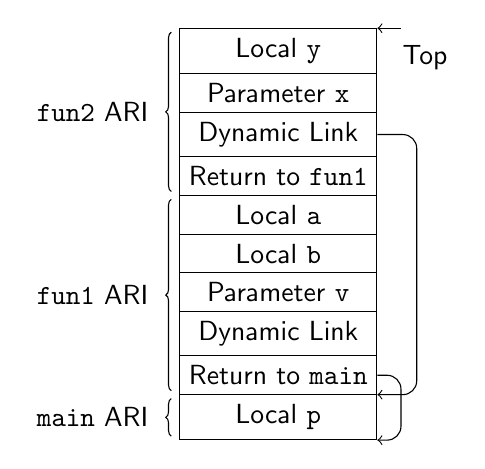
\begin{tikzpicture}[font=\sffamily,
  mystack/.style={rectangle split,rectangle split parts=#1,draw,anchor=center},
  myline/.style={->, rounded corners=5pt},
  mydec/.style={decorate,decoration={brace,amplitude=2pt}}]

  \node[mystack=10] (stk) {
    Local \texttt{y}
    \nodepart{two} Parameter \texttt{x}
    \nodepart{three} Dynamic Link
    \nodepart{four} Return to \texttt{fun1}
    \nodepart{five}Local \texttt{a}
    \nodepart{six} Local \texttt{b}
    \nodepart{seven} Parameter \texttt{v}
    \nodepart{eight} Dynamic Link
    \nodepart{nine} Return to \texttt{main}
    \nodepart{ten} Local \texttt{p}
  };

  \draw[myline] (stk.three east) -- ([xshift=.5cm]stk.three east) -- ([xshift=.5cm]stk.nine split east) -- (stk.nine split east);
  \draw[myline] (stk.nine east) -- ([xshift=.3cm]stk.nine east) -- ([xshift=.3cm]stk.south east) -- (stk.south east);

  \node [right=2cm of stk.text] (top) {Top};
  \draw[myline] ([xshift=.3cm]stk.north east) -- (stk.north east);

  \draw[mydec] ([xshift=-.1cm,yshift=.5mm]stk.four split west) --
               ([xshift=-.1cm,yshift=-.5mm]stk.north west) node [black,midway,xshift=-1cm] {\texttt{fun2} ARI};
  \draw[mydec] ([xshift=-.1cm,yshift=.5mm]stk.nine split west) --
               ([xshift=-.1cm,yshift=-.5mm]stk.four split west) node [black,midway,xshift=-1cm] {\texttt{fun1} ARI};
  \draw[mydec] ([xshift=-.1cm,yshift=.5mm]stk.south west) --
               ([xshift=-.1cm,yshift=-.5mm]stk.nine split west) node [black,midway,xshift=-1cm] {\texttt{main} ARI};

\end{tikzpicture}
\end{document}
